\section{JACO2 robotic arm}

In this section a briefly description of the JACO$^2$ robotic arm will be given. It is a 6 DOF robotic arm  with a three fingered hand developed by Kinova Robotics. It is lightweight $\left( 4.4 kg\right)$, which makes this machine specially usable in assistive and collaborative applications. It is designed to help people with upper body disabilities in order to gain more autonomy in ordinary daily tasks.\\

\begin{figure}[H]                    
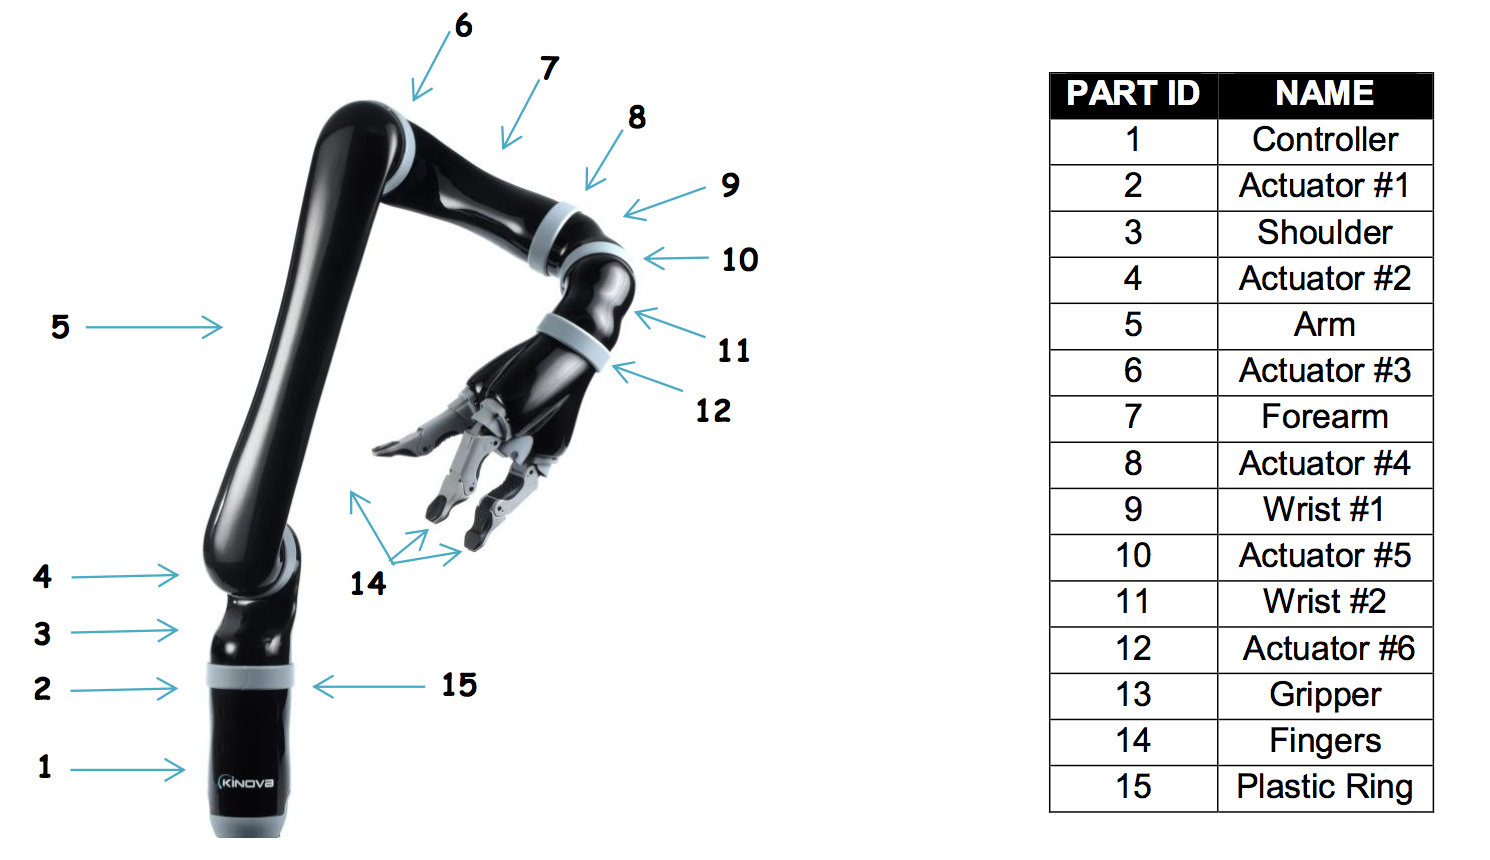
\includegraphics[width=.3\textwidth]{figures/Jaco/roboticarm}  %<--but is not needed.
\caption{6 DOF JACO$^2$ robotic arm from Kinova Robotics. \cite{kinova2017}}
\label{fig:roboticarm}  %<--give the figure a label, so you can reference!
\end{figure}
\textbf{new more exciting picture of the same thing}

The JACO$^2$ is a serial manipulator, which means that this kind of robotic arm is designed as a series of links connected by motor-actuated joints that extend from a base to an end-effector. Any movement in a joint affects all the following joints and links in the chain. The arm can by default be controlled with the help of a joystick, but it can be programmed in C++ to be controlled by other means, using the software development kit (SDK) provided by the manufacturer.\\

\textbf{include picture of JACO arm with all the names of things on/in it.}

%The control of the JACO$^2$ arm can be Angular and Cartesian. In Angular control each actuator moves separately. Cartesian robots called Gantry robots as well, are mechatronic devices which make linear movements in three axes, perpendicularly oriented to each other. It allows eight movements:
%\begin{itemize}
%\item Three translations
%\item Three rotations of the wrist
%\item Two movements of the fingers $\left( open/close\right) $
%\end{itemize}

